% Gerado automaticamente. No preambulo do documento use:
% \usepackage{pgfplots}
% \pgfplotsset{compat=1.18}
\definecolor{plotblue}{HTML}{2563EB}
\definecolor{plotorange}{HTML}{D97706}
\definecolor{plotgreen}{HTML}{059669}
\definecolor{plotpurple}{HTML}{7C3AED}
\definecolor{plotgray}{HTML}{374151}
\definecolor{plotred}{HTML}{DC2626}
\definecolor{plotteal}{HTML}{0F766E}
\definecolor{plotslate}{HTML}{64748B}

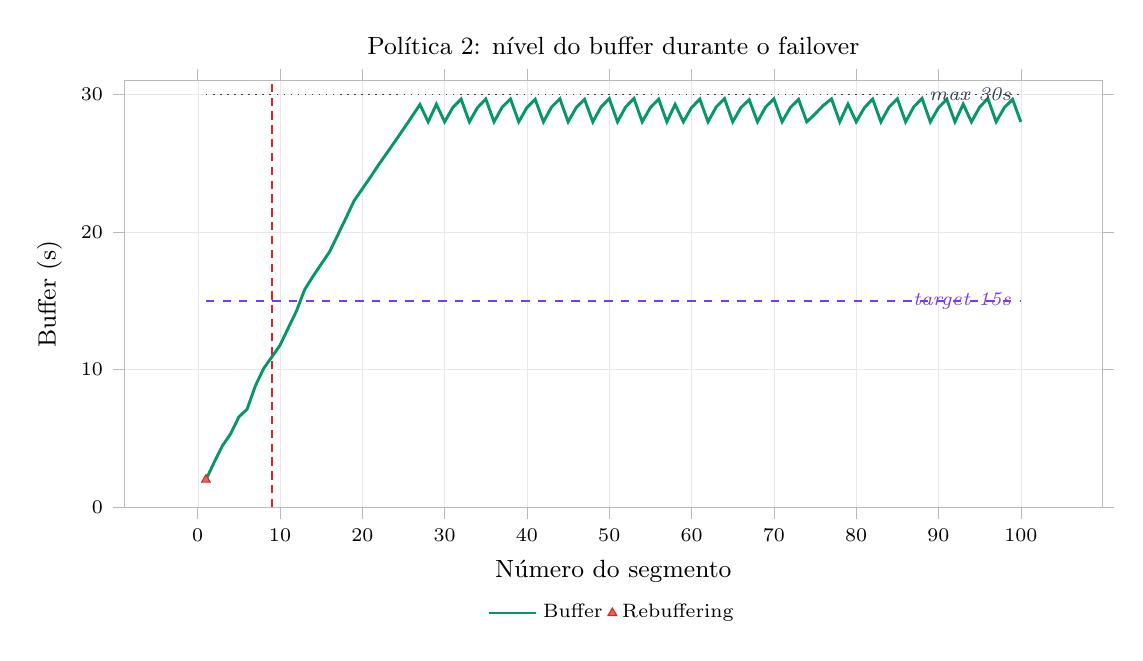
\begin{tikzpicture}
\begin{axis}[
    title={Política 2: nível do buffer durante o failover},
    xlabel={Número do segmento},
    ylabel={Buffer (s)},
    width=14cm,
    height=7cm,
    grid=major,
    grid style={line width=.12pt, draw=gray!18},
    axis line style={draw=gray!55},
    tick style={draw=gray!55},
    tick align=outside,
    title style={font=\small},
    label style={font=\small},
    tick label style={font=\scriptsize},
    legend cell align={left},
    legend style={at={(0.5,-0.20)}, anchor=north, legend columns=3, draw=none, font=\scriptsize},
    ymin=0,
    ymax=31
]
\addplot+[plotgreen, line width=1.05pt, mark=none] coordinates {
(1,2)
(2,3.26)
(3,4.46)
(4,5.34)
(5,6.56)
(6,7.12)
(7,8.81)
(8,10.07)
(9,10.91)
(10,11.77)
(11,13.02)
(12,14.26)
(13,15.82)
(14,16.77)
(15,17.66)
(16,18.54)
(17,19.76)
(18,21)
(19,22.27)
(20,23.13)
(21,24)
(22,24.9)
(23,25.75)
(24,26.61)
(25,27.48)
(26,28.36)
(27,29.26)
(28,28)
(29,29.28)
(30,28)
(31,29.05)
(32,29.65)
(33,28)
(34,29.04)
(35,29.66)
(36,28)
(37,29.08)
(38,29.66)
(39,28)
(40,29.04)
(41,29.64)
(42,28)
(43,29.08)
(44,29.68)
(45,28)
(46,29.05)
(47,29.64)
(48,28)
(49,29.08)
(50,29.69)
(51,28)
(52,29.09)
(53,29.7)
(54,28)
(55,29.04)
(56,29.65)
(57,28)
(58,29.27)
(59,28)
(60,29.04)
(61,29.65)
(62,28)
(63,29.09)
(64,29.69)
(65,28)
(66,29.04)
(67,29.61)
(68,28)
(69,29.08)
(70,29.67)
(71,28)
(72,29.04)
(73,29.63)
(74,28)
(75,28.57)
(76,29.19)
(77,29.67)
(78,28)
(79,29.29)
(80,28)
(81,29.03)
(82,29.66)
(83,28)
(84,29.08)
(85,29.68)
(86,28)
(87,29.09)
(88,29.71)
(89,28)
(90,29.03)
(91,29.64)
(92,28)
(93,29.29)
(94,28)
(95,29.07)
(96,29.69)
(97,28)
(98,29.04)
(99,29.63)
(100,28)
};
\addlegendentry{Buffer}
\addplot+[plotpurple, dashed, line width=0.55pt, mark=none, forget plot] coordinates {(1,15) (100,15)};
\node[anchor=east, plotpurple, font=\scriptsize\itshape] at (axis cs:100,15) {target 15s};
\addplot+[plotgray, dotted, line width=0.55pt, mark=none, forget plot] coordinates {(1,30) (100,30)};
\node[anchor=east, plotgray, font=\scriptsize\itshape] at (axis cs:100,30) {max 30s};
\addplot+[only marks, mark=triangle*, mark size=1.8pt, plotred, mark options={solid, fill=plotred!70, draw=plotred}] coordinates {
(1,2)
};
\addlegendentry{Rebuffering}
\addplot+[plotred, line width=0.65pt, densely dashed, mark=none, forget plot] coordinates {(9,0) (9,31)};
\end{axis}
\end{tikzpicture}
